% !TeX spellcheck = de_DE
\documentclass{article}
\usepackage{cite}
\usepackage{amsmath,amssymb,amsfonts}
\usepackage{algorithmic}
\usepackage{graphicx}
\usepackage{float} 
\usepackage{subfigure}
\usepackage{textcomp}
\usepackage{xcolor}
\usepackage{booktabs}
\usepackage{caption}
\usepackage[colorlinks]{hyperref}
\usepackage{fontspec, xunicode, xltxtra}  
\usepackage{import}
\usepackage{ctex}
\usepackage{listings}
\usepackage{fontspec} % 定制字体
\newfontfamily\menlo{Menlo}
\usepackage{xcolor} % 定制颜色
\usepackage{underscore}
\definecolor{mygreen}{rgb}{0,0.6,0}
\definecolor{mygray}{rgb}{0.5,0.5,0.5}
\definecolor{mymauve}{rgb}{0.58,0,0.82}
\lstset{ %
	backgroundcolor=\color{white},      % choose the background color
	basicstyle=\footnotesize\ttfamily,  % size of fonts used for the code
	columns=fullflexible,
	tabsize=4,
	breaklines=true,               % automatic line breaking only at whitespace
	captionpos=b,                  % sets the caption-position to bottom
	commentstyle=\color{mygreen},  % comment style
	escapeinside={\%*}{*)},        % if you want to add LaTeX within your code
	keywordstyle=\color{blue},     % keyword style
	stringstyle=\color{mymauve}\ttfamily,  % string literal style
	frame=single,
	rulesepcolor=\color{red!20!green!20!blue!20},
	% identifierstyle=\color{red},
	language=c++,
}
\usepackage{geometry}
\geometry{a4paper, scale=0.8}
\title{《Poisson Image Editing》代码阅读报告}
\author{李文彬,1120173001}
\date{\today}

\begin{document}
	\maketitle
	\section{论文概要}
	\subsection{论文要解决的问题}
    论文中提出了一种基于泊松方程的图像融合方法。泊松重建的实质是通过方程组Ax = b的求解得到融合结果的像素颜色值。图像融合算法即计算系数矩阵A和散度b.
    
    该方法可以实现前景图像和背景图像在融合边界上的较为自然过渡效果。
  
    \subsection{论文采用的主要方法}
      对于前景图像兴趣区域(ROI),计算ROI的梯度场Isrc背景图像不被修改的像素区域的梯度场Idst。然后通过对Isrc和Idst结果求和得到整幅待重建图像的梯度场,最后才根据梯度场求解散度。
      
     计算泊松方程组散度值b的流程如图\ref{fig.1}
    \begin{figure}[H]
        \centering
        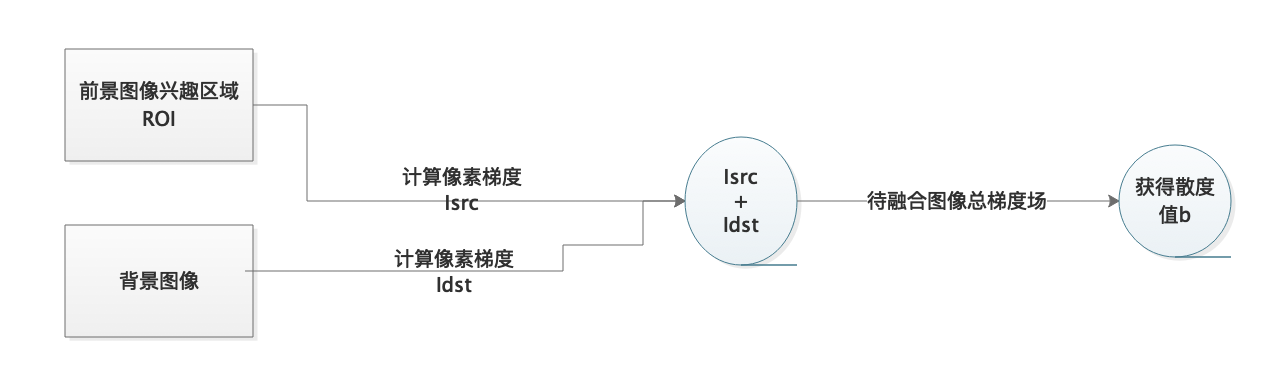
\includegraphics[width=18.0cm,height = 8.0cm]{img/b.png} 
        \caption{散度值b求解流程图}
        \label{fig.1}
    \end{figure}
\section{相关模块功能以及API调用}
本报告主要分析Seamless_clone.cpp的功能实现以及分析相关模块功能,相关API调用
\subsection{demo分析}
	\begin{lstlisting}
{/**
作用:
剪裁,无缝融合,待融合区域先剪裁

*/

#include <blend/clone.h>
#include <opencv2/opencv.hpp>

/**

Naive image cloning by just copying the values from foreground over background

*/
void naiveClone(cv::InputArray background_,
cv::InputArray foreground_,
cv::InputArray foregroundMask_,
int offsetX, int offsetY,
cv::OutputArray destination_)
{
cv::Mat bg = background_.getMat();       //背景图像
cv::Mat fg = foreground_.getMat();       //前景图像
cv::Mat fgm = foregroundMask_.getMat();  //前景mask

destination_.create(bg.size(), bg.type()); // dst兴趣区域的矩形
cv::Mat dst = destination_.getMat();

cv::Rect overlapAreaBg, overlapAreaFg;
blend::detail::findOverlap(background_, foreground_, offsetX, offsetY, overlapAreaBg, overlapAreaFg);

/**
前景图片 矩形中图像  转到背景图片中

*/
bg.copyTo(dst);
fg(overlapAreaFg).copyTo(dst(overlapAreaBg), fgm(overlapAreaFg));

}

/**

Main entry point.

*/
int main(int argc, char **argv)
{
if (argc != 6) {
std::cerr << argv[0] << " background foreground mask offsetx offsety" << std::endl;
return -1;
}

cv::Mat background = cv::imread(argv[1]);
cv::Mat foreground = cv::imread(argv[2]);
cv::Mat mask = cv::imread(argv[3], CV_LOAD_IMAGE_GRAYSCALE);
int offsetx = atoi(argv[4]);
int offsety = atoi(argv[5]);


cv::Mat result;

naiveClone(background, foreground, mask, offsetx, offsety, result);
cv::imshow("Naive", result);
cv::imwrite("naive.png", result);

/**
* 输出融合结果
* 步骤一 :计算组合梯度场
*          mixed  
*          保留destination 图像的texture 细节
*          目标区域的梯度是由原图像和目的图像的组合计算出来(计算gradient)。
* 步骤二 :计算背景图片梯度场
* 步骤三 :计算平均梯度场
*/

blend::seamlessClone(background, foreground, mask, offsetx, offsety, result, blend::CLONE_MIXED_GRADIENTS);
cv::imshow("Mixed Gradients", result);
cv::imwrite("mixed-gradients.png", result);

blend::seamlessClone(background, foreground, mask, offsetx, offsety, result, blend::CLONE_FOREGROUND_GRADIENTS);
cv::imshow("Foreground Gradients", result);
cv::imwrite("foreground-gradients.png", result);

blend::seamlessClone(background, foreground, mask, offsetx, offsety, result, blend::CLONE_AVERAGED_GRADIENTS);
cv::imshow("Averaged Gradients", result);
cv::imwrite("averaged-gradients.png", result);

cv::waitKey();

return 0;
}
}
\end{lstlisting}

    \subsection{功能实现分析}
    现假设有一图像g,如图\ref{fig.2}
      \begin{figure}[H]
    	\centering
    	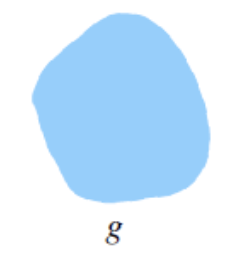
\includegraphics[width=0.2\textwidth]{img/ROI.png}
    	\caption{待克隆图像ROI}
    	\label{fig.2}
    \end{figure}
有一背景图片S,如图\ref{fig.3}
\begin{figure}[H]
	\centering
	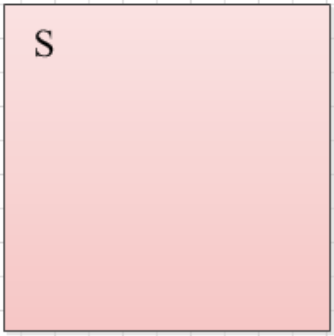
\includegraphics[width=0.2\textwidth]{img/R.png}
	\caption{背景图片R}
	\label{fig.3}
\end{figure}    
融合目标即为把图片G融合粘贴到s中,且实现自然粘贴的效果,如图\ref{fig.4}
\begin{figure}[H]
	\centering
	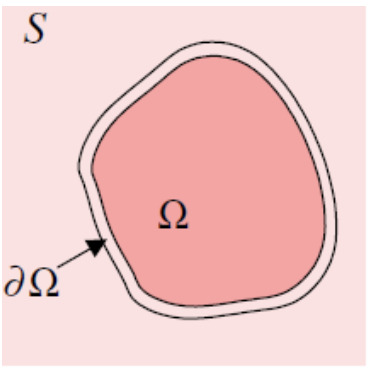
\includegraphics[width=0.2\textwidth]{img/Clone.png}
	\caption{融合后图片}
	\label{fig.4}
\end{figure}    
    \subsection{算法实现
    	\\——与Seamless_cloning.cpp相关的OpenCV函数库及API分析}
    \subsubsection{计算前景图像ROI的梯度场}
    通过差分方法,可以求得图像g的梯度场。
    OpenCV中泊松融合计算g梯度场的代码如下:
    \begin{lstlisting}
    void Cloning::computeGradientX( const Mat &img, Mat &gx)
    {
    Mat kernel = Mat::zeros(1, 3, CV_8S);
    kernel.at<char>(0,2) = 1;
    kernel.at<char>(0,1) = -1;
    
    if(img.channels() == 3)
    {
    filter2D(img, gx, CV_32F, kernel);
    }
    else if (img.channels() == 1)
    {
    Mat tmp[3];
    for(int chan = 0 ; chan < 3 ; ++chan)
    {
    filter2D(img, tmp[chan], CV_32F, kernel);
    }
    merge(tmp, 3, gx);
    }
    }
    
    void Cloning::computeGradientY( const Mat &img, Mat &gy)
    {
    Mat kernel = Mat::zeros(3, 1, CV_8S);
    kernel.at<char>(2,0) = 1;
    kernel.at<char>(1,0) = -1;
    
    if(img.channels() == 3)
    {
    filter2D(img, gy, CV_32F, kernel);
    }
    else if (img.channels() == 1)
    {
    Mat tmp[3];
    for(int chan = 0 ; chan < 3 ; ++chan)
    {
    filter2D(img, tmp[chan], CV_32F, kernel);
    }
    merge(tmp, 3, gy);
    }
    }
    
   \end{lstlisting}
    通过上述代码,可以得到函数返回值V(pathGradientX,VpatchGradientY),
    相关函数调用API如下:
    \begin{lstlisting}
    computeGradientX(patch,patchGradientX);//计算ROI区域转换复制到destination一样大小的patch图片x方向梯度
    computeGradientY(patch,patchGradientY);//计算y方向梯度
    \end{lstlisting}
 

    \subsubsection{计算背景图片的梯度场}
     与前景图像计算同理,可以得到背景图片和融合图片的梯度场,函数调用API如下:
    \begin{lstlisting}
       
    computeGradientX(destination,destinationGradientX);//计算背景图像的x方向梯度
    computeGradientY(destination,destinationGradientY);//计算背景图像y方向的梯度
    \end{lstlisting}
    \subsubsection{计算融合图像的梯度场}
    \begin{lstlisting}
    Mat laplacianX = Mat(destination.size(),CV_32FC3);
    Mat laplacianY = Mat(destination.size(),CV_32FC3);
    
    //因为前面已经对destinationGradientX做了固定区域的mask,patchGradientX做了修改区域的mask
    laplacianX = destinationGradientX + patchGradientX;//求解整张图片新的梯度场
    laplacianY = destinationGradientY + patchGradientY;
    
    \end{lstlisting}
    
%    \begin{figure}[H]
%        \centering
%        \includegraphics[width=0.75\textwidth]{img/CircleMatch.png}
%        \caption{环形匹配过程}
%        \label{fig.2}
%    \end{figure}
%    \begin{figure}[H]
%        \centering
%        \includegraphics[width=0.75\textwidth]{img/CircleMatchOrNot.png}
%        \caption{环形匹配是否成功}
%        \label{fig.3}
%    \end{figure}
    \subsubsection{求解融合图像散度}
    对拉普拉斯算子在x和y方向求偏导,求和;
   \begin{lstlisting}
    lap = laplacianX + laplacianY;//散度
   \end{lstlisting}
    
    \section{实验运行}
    由于原始版C++demo使用不熟练,因此选择运行开源的Python版demo,但针对实验结果API给出C++版本的解释
    \\   开源链接:
    \href{https://www.learnopencv.com/seamless-cloning-using-opencv-python-cpp/}{	https://www.learnopencv.com/seamless-cloning-using-opencv-python-cpp/}
    \subsection{Python版本}
    可运行程序:
    \begin{lstlisting}
    # 注意修改路径!
    import cv2
    import numpy as np
    
    # Read images : src image will be cloned into dst
    im = cv2.imread("images/wood-texture.jpg")
    obj= cv2.imread("images/iloveyouticket.jpg")
    
    # Create an all white mask
    mask = 255 * np.ones(obj.shape, obj.dtype)
    
    # The location of the center of the src in the dst
    width, height, channels = im.shape
    center = (height/2, width/2)
    
    # Seamlessly clone src into dst and put the results in output
    normal_clone = cv2.seamlessClone(obj, im, mask, center, cv2.NORMAL_CLONE)
    mixed_clone = cv2.seamlessClone(obj, im, mask, center, cv2.MIXED_CLONE)
    
    # Write results
    cv2.imwrite("images/opencv-normal-clone-example.jpg", normal_clone)
    cv2.imwrite("images/opencv-mixed-clone-example.jpg", mixed_clone)
    \end{lstlisting}
%    \begin{figure}[H]
%        \centering
%        \includegraphics[width=0.8\textwidth]{img/matlab.png} 
%        \caption{matlab版程序运行结果}
%        \label{fig.4}
%    \end{figure}
\subsection{API解释}
\subsubsection{C++版本}
\begin{lstlisting}
blend::seamlessClone(background, foreground, mask, offsetx, offsety, result, blend::CLONE_MIXED_GRADIENTS);
//or
blend::seamlessClone(background, foreground, mask, offsetx, offsety, result, blend::CLONE_FOREGROUND_GRADIENTS);
//or
blend::seamlessClone(background, foreground, mask, offsetx, offsety, result, blend::CLONE_AVERAGED_GRADIENTS);
\end{lstlisting}
	
	\begin{tabular}{cc}
		\hline
		foreground& 目标影像 \\
		\hline
		background& 背景图片\\
		\hline
		mask& 表示目标影像上的ROI\\
		\hline
		offsetx& 目标影像中心在背景图片上x坐标  \\
		\hline
		offsety& 目标影像中心在背景图片上y坐标 \\
		\hline
		result& 输出图像 \\
		\hline
		blend::&模式选择\\
	\end{tabular}
	

\subsubsection{Python版本}
\begin{lstlisting}
output = cv2.seamlessClone(src, dst, mask, center, flags)
\end{lstlisting}

(同名参数以及简单命名参数与C++版本比较,易得类似API解释)\\ \\
\begin{tabular}{cc}
	\hline
	center& 目标影像中心在背景图片上坐标\\
	\hline
	flags& 模式选择\\
	\hline
	\end{tabular}


    \subsection{运行实例}
    前景图像
    \begin{figure}[H]
        \centering
        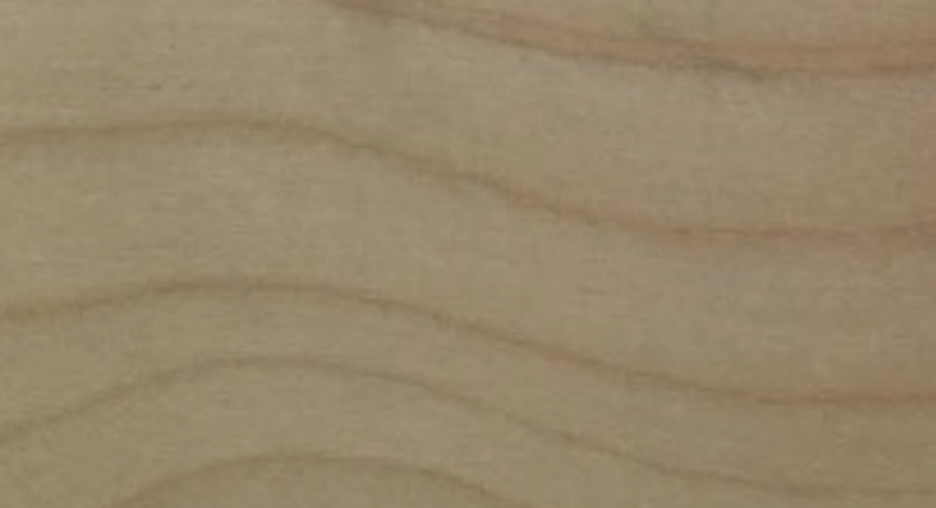
\includegraphics[width=0.4\textwidth]{img/back.png} 
        \caption{前景图像}
        \label{fig.5}
    \end{figure}
  背景图片
\begin{figure}[H]
	\centering
	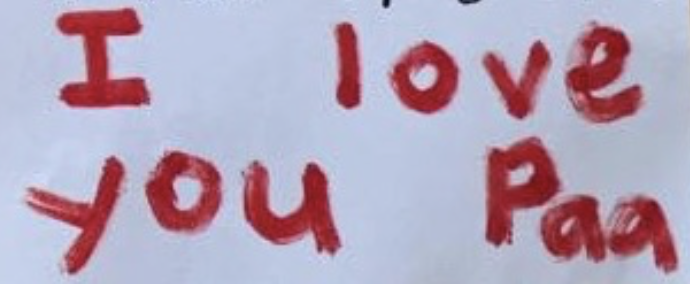
\includegraphics[width=0.4\textwidth]{img/front.png} 
	\caption{背景图片}
	\label{fig.6}
\end{figure}   
  前景图像
\begin{figure}[H]
	\centering
	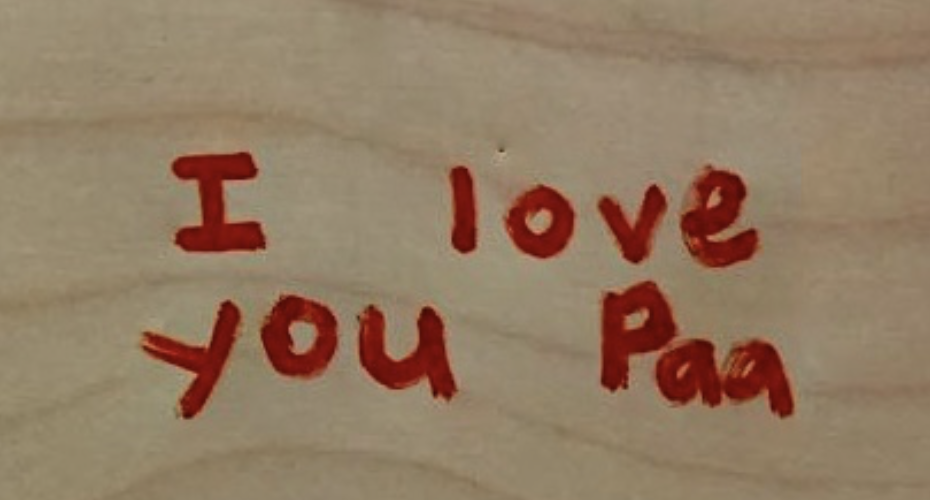
\includegraphics[width=0.4\textwidth]{img/result.png} 
	\caption{融合图片}
	\label{fig.7}
\end{figure}
\end{document}